\documentclass[10pt,a4paper]{article}
\usepackage[utf8]{inputenc}
\usepackage{multirow}
\usepackage{amsmath}
\usepackage{amsfonts}
\usepackage{amssymb}
\usepackage{graphicx}
\usepackage{pstricks-add}
\usepackage{auto-pst-pdf}
\usepackage{pst-pdf}
\usepackage[left=2cm,right=2cm,top=2cm,bottom=2cm]{geometry}

\renewcommand{\figurename}{Obrázek}
\def\doubleunderline#1{\underline{\underline{#1}}}

\begin{document}
    \begin{center}
       {\Large \textbf{VYSOKÉ UČENÍ TECHNICKÉ V BRNĚ}}
       \\[18pt]
       {\huge  Fakulta informačních technologií}
       \\[220pt]
       {\LARGE  ELEKTRONIKA PRO INFORMAČNÍ TECHNOLOGIE}
       \\[20pt]
       {\LARGE  2017/2018}
       \\[40pt]
       {\LARGE \textbf{ SEMESTRÁLNÍ PROJEKT}}
       \\[320pt]
    \end{center}
    
    \begin{flushleft}
        \begin{large}
         Tomáš Tlapák (xtlapa00) \hfill  20. prosince 2017
        \end{large}
    \end{flushleft}
   
   \begin{flushleft}
    {\large 1. příklad}
    \\[10pt]
    Postup: Obvod postupně zjednodušujeme a zpětně dopočítáváme hodnoty veličin pomocí Ohmova zákona a Kirchhoffových zákonů.
    \\[15pt]
   \end{flushleft}
   
   \begin{figure}[ht]
    \begin{center}
     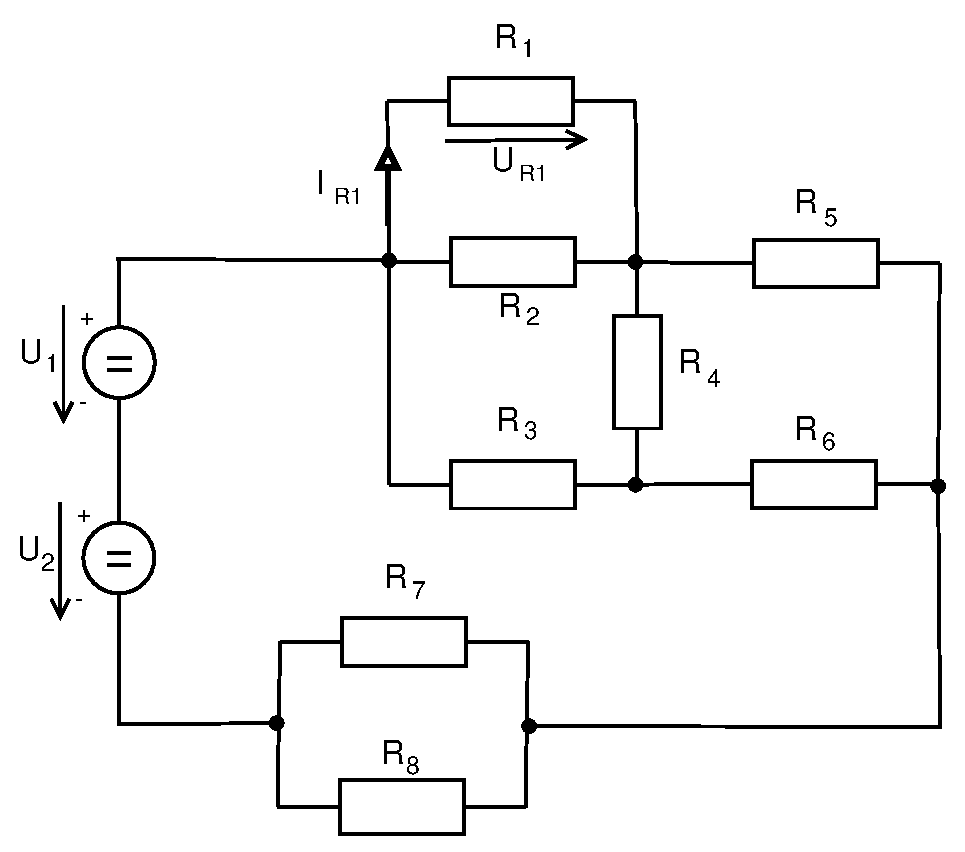
\includegraphics[width=0.6\textwidth]{2017.eps}
     \caption{schéma obvodu}
    \end{center}
   \end{figure}
  
   \begin{center}
    \begin{large}
      $ U_{12} = U_1 + U_2 = 115 + 55 = 170$ V \\[6pt]
      $ R_{12} = \dfrac{R_1 \cdot {R_2}}{R_1  +R_2} = \dfrac{485\cdot 660}{485+660} = 279.5633 $ $\Omega$ \\[6pt]
      $ R_{78} = \dfrac{R_7 \cdot {R_8}}{R_7 + R_8} = \dfrac{255\cdot 225}{255 + 225} = 119,5312 $ $\Omega$ \\[20pt]
    \end{large}
   \end{center}
  
   \begin{figure}[ht]
    \begin{center}
     \includegraphics[width=0.6\textwidth]{2018.eps}
      \caption{schéma obvodu}
    \end{center}
   \end{figure}
   \newpage
   
    
    \begin{center}
     \begin{large}
      $ R_A = \dfrac{R_{12} \cdot {R_3}}{R_{12}+R_3+R_4} = \dfrac{279.5633 \cdot100}{279.5633+100+340} = \dfrac{27956.3300}{719.5633} = 38.8518 $  $\Omega$
      \\[6pt]
      $ R_B = \dfrac{R_{12} \cdot {R_4}}{R_{12}+R_3+R_4} = \dfrac{279.5633 \cdot340}{279.5633+100+340} = \dfrac{95051.5220}{719.5633} = 132.0961 $  $\Omega$
      \\[6pt]
      $ R_C = \dfrac{R_3 \cdot {R_4}}{R_{12}+R_3+R_4} = \dfrac{100 \cdot340}{279.5633+100+340} = \dfrac{34000}{719.5633} = 47.2508 $  $\Omega$
      \\[20pt]
   \end{large}
  \end{center} 
  
   \begin{figure}[ht]
    \begin{center}
     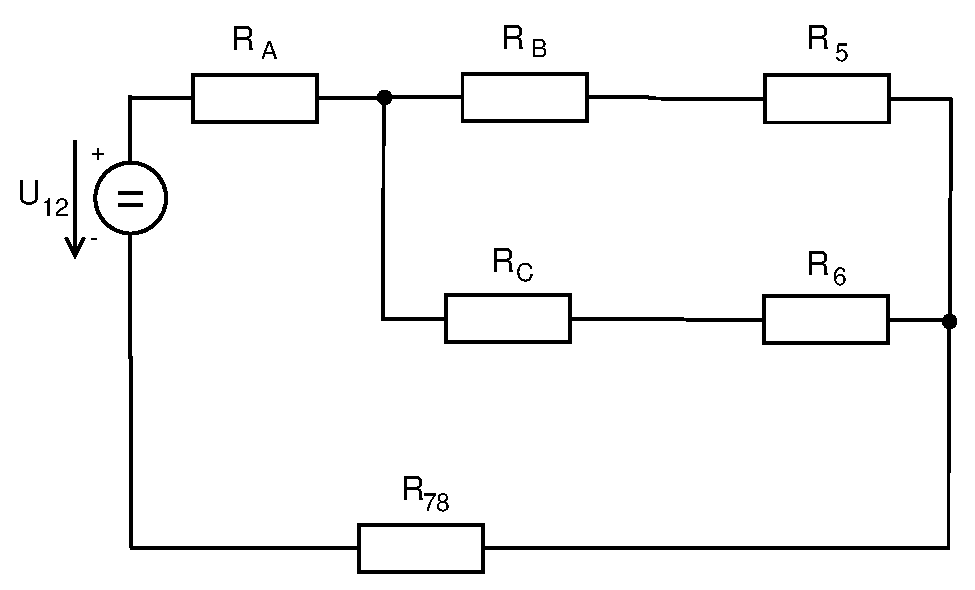
\includegraphics[width=0.6\textwidth]{2019.eps}
      \caption{schéma obvodu}
    \end{center}
   \end{figure} 

    \begin{center}
     \begin{large}
      $ R_{B5} = R_B+R_5 = 132.0961+575 = 707,0961 $  $\Omega$
      \\[6pt]
      $ R_{C6} = R_C+R_6 = 47.2508+815 = 862,2508 $  $\Omega$
      \\[20pt]    
   \end{large}
  \end{center} 
  
  \begin{figure}[ht]
    \begin{center}
     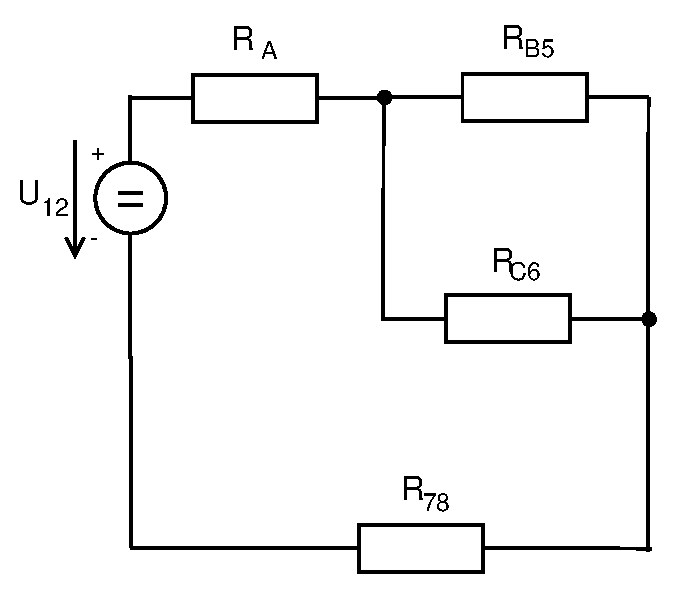
\includegraphics[width=0.5\textwidth]{2020.eps}
      \caption{schéma obvodu}
    \end{center}
   \end{figure} 
   \newpage
  
  \begin{center}
     \begin{large}
      $ R_{B5C6} =\dfrac {R_{B5}\cdot R_{C6}}{R_{B5}+R_{C6}}= \dfrac{707.0961\cdot 862.2508}{707.0961+862.2508} = \dfrac{609694.1779}{1569.3469} = 388.5018 $ $\Omega$
      \\[6pt]
      $ R_{EKV} = R_A+R_{B5C6}+R_{78}= 38.8518 + 388.5018 +119.5312 = 546.8848 $ $\Omega$
      \\[6pt]
      $ I = \dfrac{U_{12}}{R_{EKV}} = \dfrac{170}{546.8848} = 0.3108 $ A 
      \\[6pt]
      $ U_{R_A} = R_A \cdot I = 38.8518 \cdot 0.3108 = 12.0751 $ V
      \\[6pt]
      $ U_{R_{B5C6}} = R_{B5C6} \cdot I = 388.5018 \cdot 0.3108 = 120.7463 $ V
      \\[6pt]
      $  U_{R_{78}} = R_{78} \cdot I = 119.5312 \cdot 0.3108 = 37.1502  $ V 
      \\[20pt]    
   \end{large}
  \end{center} 

  \begin{figure}[ht]
    \begin{center}
     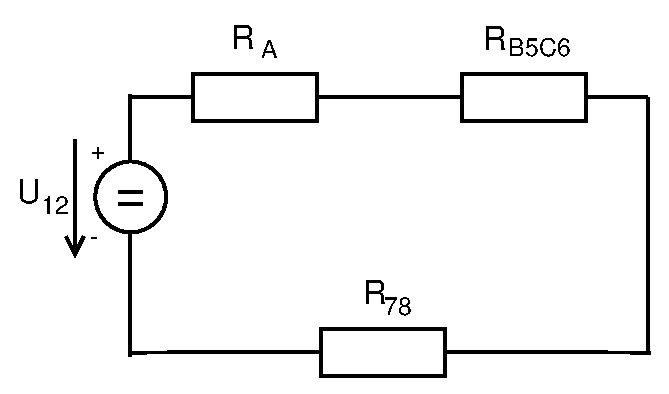
\includegraphics[width=0.6\textwidth]{2021.eps}
      \caption{schéma obvodu}
    \end{center}
   \end{figure}  

    \begin{center}
     \begin{large}
      $ I_{R_{B5}}=\dfrac{U_{R_{B5C6}}}{R_{B5}}  = \dfrac{120.7463}{707.0961} =0.1707 $ A
      \\[6pt]
     $ I_{R_{C6}}=\dfrac{U_{R_{B5C6}}}{R_{C6}}  = \dfrac{120.7463}{862.2508} =0.1400 $ A
     \\[20pt]
   \end{large}
  \end{center}
  
  \begin{figure}[ht]
    \begin{center}
     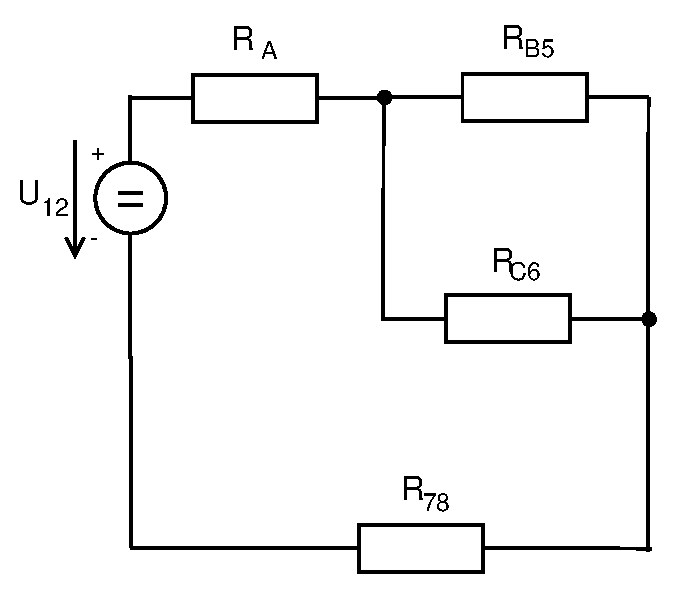
\includegraphics[width=0.523\textwidth]{2020.eps}
      \caption{schéma obvodu}
    \end{center}
   \end{figure}   
   \newpage  
   
   \begin{center}
     \begin{large}
      $ U_{R_B} = R_B \cdot I_{R_{B5}}=132.0961 \cdot 0.1707  =22.5488 $ V
      \\[6pt]
      $ U_{R_5}= R_5 \cdot I_{R_{B5}}=575 \cdot 0.1707  =98.1525 $ V
      \\[6pt]
      $ U_{R_C}= R_C \cdot I_{R_{C6}}=47.2508  \cdot 0.1400  =6.6151 $ V
      \\[6pt]
      $ U_{R_6}= R_6 \cdot I_{R_{C6}}=815 \cdot 0.1400  =114.1000 $ V
     \\[20pt]
   \end{large}
  \end{center}
   
   \begin{figure}[ht]
    \begin{center}
     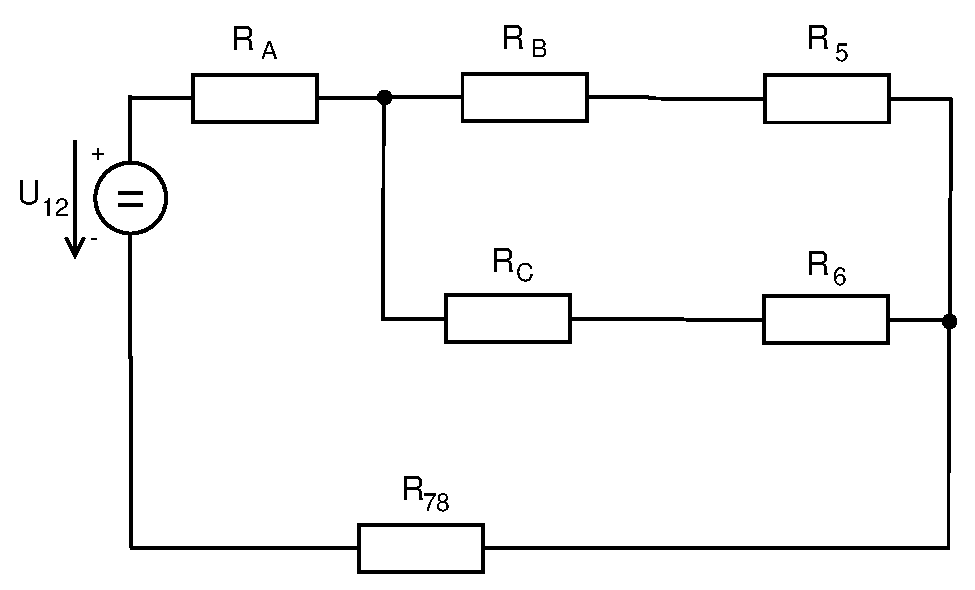
\includegraphics[width=0.6\textwidth]{2019.eps}
      \caption{schéma obvodu}
    \end{center}
   \end{figure} 
   
   \begin{center}
     \begin{large}
      $ U_{R_4} + U_{R_5} - U_{R_6} = 0$
      \\[6pt]
      $ U_{R_4} = U_{R_6} - U_{R_5} = 114,1000 - 98,1525 = 15,9475 $ V
      \\[6pt]
      $ I_{R_4} = \dfrac{U_{R_4}}{R_4} = \dfrac{15,9475}{340} = 0.0469  $ A
      \\[20pt]
      $ I_{R_3} = I_{R_4} +  I_{R_{C6}} =0.0469 + 0.1400 = 0.1869  $ A
      \\[6pt]
      $ U_{R_3}= R_3 \cdot I_3=100 \cdot 0.1869  =18.6900 $ V
      \\[20pt]
   \end{large}
  \end{center}
  
  \begin{figure}[ht]
    \begin{center}
     \includegraphics[width=0.6\textwidth]{2018.eps}
      \caption{schéma obvodu}
    \end{center}
   \end{figure}
   \newpage
   
   \begin{center}
     \begin{large}
      $ U_{R_{12}} -  U_{R_4} - U_{R_3} =  0 $
      \\[6pt]
      $ U_{R_{12}} =  U_{R_4} + U_{R_3}$
      \\[6pt]
      $ U_{R_{12}} = U_{R_1} = U_{R_2} =  U_{R_4} + U_{R_3} = 15.9475 + 18.6900 = \doubleunderline{34.6375} $ V
      \\[6pt]
      $ I_{R_1} = \dfrac{U_{R_1}}{R_1} = \dfrac {34.6375}{485} = \doubleunderline{0.0714} $ A    
   \end{large}
  \end{center}
  
\begin{figure}[ht]
    \begin{center}
     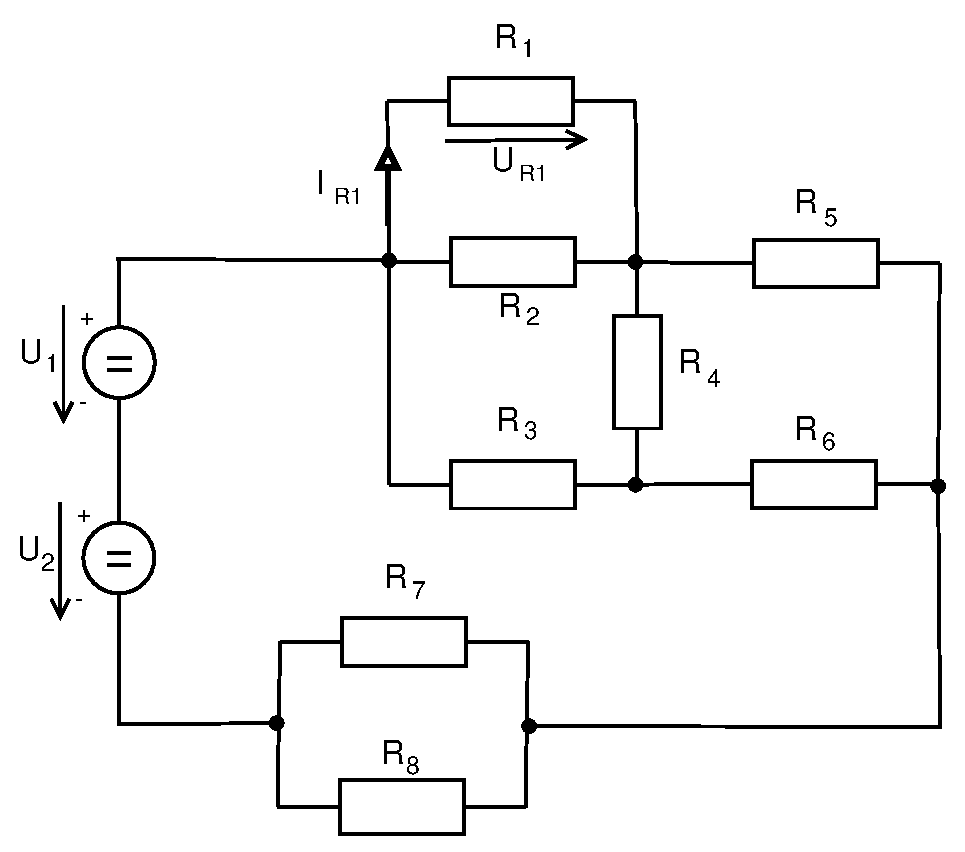
\includegraphics[width=0.6\textwidth]{2017.eps}
     \caption{schéma obvodu}
    \end{center}
   \end{figure}  
   \newpage
   
    \begin{flushleft}
    {\large 2. příklad}
    \\[10pt]
    Postup: Obvod zjednodušíme. Prvek, který chceme analyzovat odstraníme ze svorek a spočítáme proud a napětí v obvodu. Poté nahradíme zdroj vnitřní impedancí a spočítáme odpor na svorkách. Odpor a napětí mezi svorkami bude tvořit nový obvod, do kterého vrátíme předtím odebraný prvek.
    \\[15pt]
    \end{flushleft}
   
   \begin{figure}[ht]
    \begin{center}
     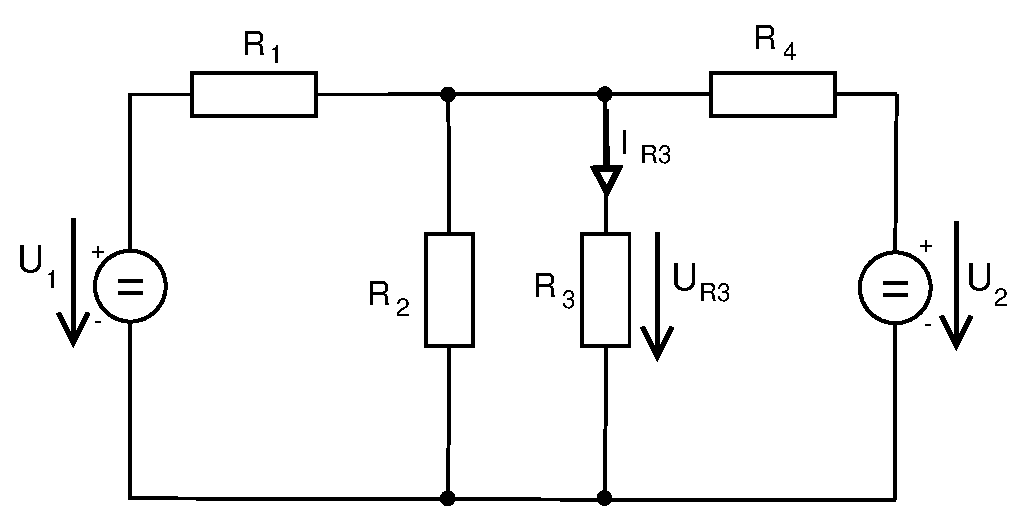
\includegraphics[width=0.6\textwidth]{2022.eps}
     \caption{schéma obvodu}
    \end{center}
   \end{figure}   
    
   
  \begin{center}
   \begin{large}
   $ R_{23} = \dfrac{R_2 \cdot R_3}{R_2 + R_3} = \dfrac{205 \cdot 580}{205 + 580} = \dfrac{118900}{785} = 151.4649$ $\Omega $
   \\[6pt]
   $ I = \dfrac{U_1 - U_2}{R_1 + R_4} = \dfrac{220 - 190}{360 + 560} = 0.0326 $ A
   \\[6pt]
   $ U_{R_{1}} = R_{1} \cdot I = 360 \cdot 0.0326 = 11.7360  $ V
   \\[20pt]  
   \end{large}
  \end{center}

\begin{figure}[ht]
    \begin{center}
     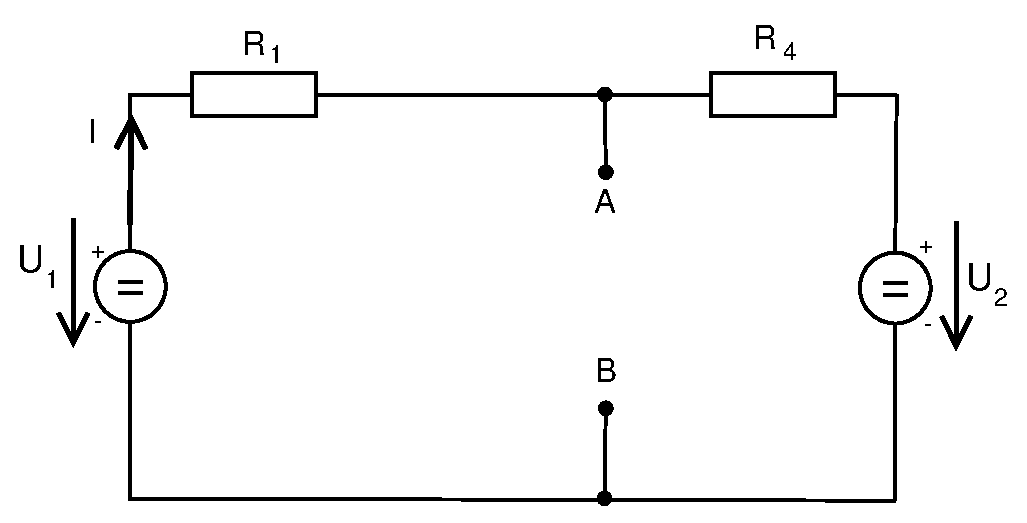
\includegraphics[width=0.6\textwidth]{2023.eps}
     \caption{schéma obvodu}
    \end{center}
   \end{figure}   
   \newpage 
  
  \begin{center}
   \begin{large}
   $ U_{THE} = U_1 - U_{R_1} = 220 - 11.7360 = 208.2640  $ V 
   \\[6pt]
   $ R_{THE} = \dfrac{R_1 \cdot R_4}{ R_1 +R_4}= \dfrac{360 \cdot 560}{360 + 560} =219.1304  $ $\Omega $ 
   \\[6pt]
   $ I_{THE} = \dfrac{U_{THE}}{R_{THE} + R_{23}} = \dfrac{208.2640}{219.1304 + 151.4649}  = 0.5619  $ A 
   \end{large}
  \end{center}
  
  \begin{figure}[ht]
    \begin{center}
     \includegraphics[width=0.6\textwidth]{2024.eps}
     \caption{schéma obvodu}
    \end{center}
   \end{figure} 
  
   \begin{center}
   \begin{large}
   $ U_{R_2} - U_{R_3} = 0 $
   \\[6pt]
   $ U_{R_2} = U_{R_3} = U_{R_{23}} $
   \\[6pt]
   $ U_{R_{23}} = I_{THE} \cdot R_{23} = 0.5619 \cdot 151.4649 = \doubleunderline{85.1081} $ V
   \\[6pt]
   $I_3 = \dfrac{U_3}{R_3} = \dfrac{85.1081}{205} = \doubleunderline{0.4151} $ A 
   \\[20pt]
   \end{large}
  \end{center}
  
  \begin{figure}[ht]
    \begin{center}
     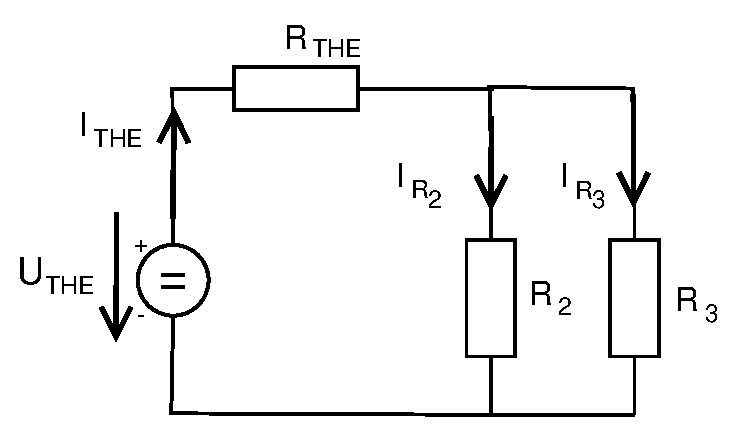
\includegraphics[width=0.6\textwidth]{2025.eps}
     \caption{schéma obvodu}
    \end{center}
   \end{figure} 
  \newpage
  
   \begin{flushleft}
    {\large 3. příklad}
    \\[10pt]
    Postup: Zdroje napětí převedeme na zdroje proudu. Odpory přepočteme na vodivost. Zvolíme referenční uzel a zakreslíme nezávislé uzly vzhledem k referenčnímu. Sestaví rovnice pro proudy v uzlech podle Kirchhoffova zákona a vypočítáme neznáme veličiny.
   \\[15pt]
    \end{flushleft}
  
 \begin{figure}[ht]
    \begin{center}
     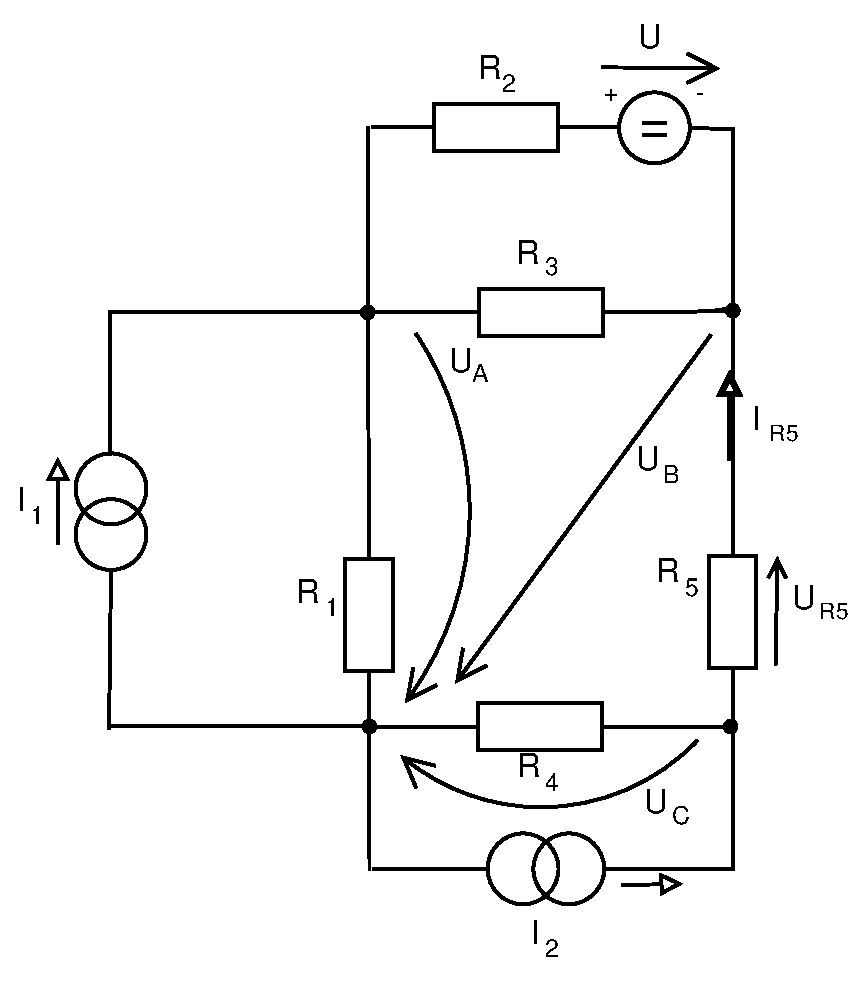
\includegraphics[width=0.6\textwidth]{2027.eps}
     \caption{schéma obvodu}
    \end{center}
   \end{figure}   

\begin{center}
   \begin{large}
   $ I_{R_3} = \dfrac{U}{R_2} = \dfrac{120}{49} = 2.4489 $ A
   \\[6pt]
   $ G_1 = \dfrac{1}{R_1} = \dfrac{1}{53} = 0.0188 $ S
   \\[6pt]
   $ G_2 = \dfrac{1}{R_2} = \dfrac{1}{49} = 0.0204 $ S
   \\[6pt]
   $ G_3 = \dfrac{1}{R_3} = \dfrac{1}{65} = 0.0153 $ S
   \\[6pt]
   $ G_4 = \dfrac{1}{R_4} = \dfrac{1}{39} = 0.0256 $ S
   \\[6pt]
   $ G_5 = \dfrac{1}{R_5} = \dfrac{1}{32} = 0.0312 $ S
   \end{large}
  \end{center}  
  \newpage
  
   \begin{figure}[t]
    \begin{center}
     \includegraphics[width=0.6\textwidth]{2026.eps}
     \caption{schéma obvodu}
    \end{center}
   \end{figure}   

   \begin{large}
    \begin{flushleft}
     Podle Kirchoffova zákona vytvoříme rovnice proudů v jednotlivých uzlech:
    \end{flushleft}
    \end{large}
   
   \begin{center}
   \begin{large}
     $ U_A \cdot (G_1 +G_2 +G_3) + U_B \cdot (-G_2 -G_3) = I_1 + I_3 $
     \\[6pt]
     $ U_A \cdot (-G_2 -G_3) + U_B \cdot (G_2 +G_3 +G_5) - U_C \cdot(-G_5) =-I_3 $   
    \\[6pt]
     $ U_B \cdot (-G_5) + U_C \cdot (G_4 + G_5) = I_2 $
     \\[40pt]
   \end{large}
  \end{center}    
  
\begin{large}
    \begin{flushleft}
     Z těchto rovnic sestavíme matici:
    \end{flushleft}
    \end{large}  
  
 \begin{center}
   \begin{large}
\[\left( 
  \begin{array}{cccc}
   \ & U_A & U_B & U_C \\
   U_A & G_1 + G_2 + G_3 & -G_2 -G_3 & 0 \\
   U_B & -G_2 - G_3 & G_2 + G_3 + G_5 & -G_5 \\
   U_C & 0 & -G_5 &G_4 +G_5 \\
  \end{array}  \right)= \begin{pmatrix} I_1 +I_3 \\ -I_3 \\ I_2 \end{pmatrix}
  .\]
  \\[20pt]         
   \end{large}
  \end{center}    
  \newpage
  
\begin{large}
    \begin{flushleft}
     Vypočteme determinant matice:
    \end{flushleft}
    \end{large}    
  
  \begin{center}
   \begin{large}
\[det M = \left| 
  \begin{array}{ccc}
    G_1 + G_2 + G_3 & -G_2 -G_3 & 0 \\
    -G_2 - G_3 & G_2 + G_3 + G_5 & -G_5 \\
    0 & -G_5 &G_4 +G_5 \\
  \end{array}  \right|=.\]  
 \[ = \left| 
  \begin{array}{ccc}
   \\\
    0.0188+ 0.0204+ 0.0153 & -0.0204 -0.0153 & 0 \\
   -0.0204 - 0.0153 & 0.0204 + 0.0153 + 0.0312 & -0.0312 \\
   0 & -0.0312 &0.0256 +0.0312 \\
  \end{array}  \right|=.\]
  \[ = \left| 
  \begin{array}{ccc}
   \\\
    0.0545& -0.0357& 0 \\
   -0.0357& 0.0669 & -0.0312 \\
   0 & -0.0312 &0.0568 \\
  \end{array}  \right|=\]
   \\[6pt]
   $= 0.0545 \cdot 0.0669 \cdot 0.0568 + (-0.0357) \cdot (-0.0312) \cdot 0+ 0\cdot (-0.0357) \cdot (-0.0312) -$ \\ $0\cdot 0.0669 \cdot 0 -(-0.0312)\cdot (-0.0312) \cdot 0.0545 - 0.0568\cdot (-0.0357)\cdot (-0.0357)= 0.000081652128 $
  \\[20pt]      
   \end{large}
  \end{center}  
 
   \begin{large}
    \begin{flushleft}
     Použijeme Cramerovo pravidlo pro výpočet $U_B$ a $U_C$, které potřebujeme pro výpočet $U_{R_5}$ a $I_{R_5}$. Postupujeme tak, že pro napětí $U_B$ nahradíme daný sloupec v matici za $\begin{pmatrix} I_1 +I_3 \\ -I_3 \\ I_2 \end{pmatrix}$ a Sarrusovým pravidlem spočítáme determinant. Výsledek podělíme $det M$ a dostaneme $U_B$. Stejně postupujeme i pro $U_C$.
    \\[20pt]
    \end{flushleft}
    \end{large}      
  
\begin{center}
   \begin{large}
   $U_B=\dfrac{\begin{vmatrix} G_1+G_2 + G_3 & I_1 +I_3 &0 \\-G_2 -G_3 & -I_3 & -G_5 \\0 & I_2 & G_4 + G_5 \end{vmatrix}}{det M} =\dfrac{\begin{vmatrix} 0.0545 & 3.3489 &0 \\-0.0357 & -2.4489 & -0.0312 \\0 & 0.7 &0.0568 \end{vmatrix}}{0.000081652128} = $
   \\[6pt]
   $\dfrac{0.0545 \cdot (-2.4489)\cdot0.0568- 0.7\cdot (-0.0312) \cdot 0.0545 -0.0568 \cdot (-0.0357)\cdot 3.3489}{0.000081652128} = $
   \\[10pt] 
   $ =\dfrac{0.000400230624}{0.000081652128} =4.9016$ V
   \\[20pt]
   $U_C=\dfrac{\begin{vmatrix} G_1+G_2 + G_3 & -G_2 -G_3 &I_1 +I_3 \\-G_2 -G_3 & G_2+ G_3+ G_5 & -I_3  \\0 &-G_5 & I_2  \end{vmatrix}}{det M} =\dfrac{\begin{vmatrix} 0.0545 & -0.0357 &3.3489 \\-0.0357 & 0.0669 &  -2.4489 \\0 & -0.0312 &0.7 \end{vmatrix}}{0.000081652128} = $
   \\[10pt]
   $=\dfrac {0.0545 \cdot 0.0669 \cdot 0.7 + 3.3489 \cdot (-0.0357) \cdot (-0.0312)-(-0.0312) \cdot (-2.44890) \cdot (0.0545)}{0.000081652128} -  $   
   \\[10pt]
   $\dfrac{ 0.7 \cdot (-0.0357)\cdot(-0.0357)}{0.000081652128} = \dfrac{0.001226121216}{0.000081652128} = 15.0164 $ V
   \\[12pt]
   $|U_{R_5}| = |U_B - U_C| = |15.0164 - 4.9016| = \doubleunderline{10,1148} $ V
   \\[8pt]
   $ I_{R_5} = \dfrac{U_{R_5}}{R_5} = \dfrac{10.1148}{32} = \doubleunderline{0.3160} $ A
   \end{large}
  \end{center}    
  \newpage
  
  \begin{center}
   \begin{large}
   \textbf{{\LARGE Tabulka hodnot}}
    
    \begin{table}[ht]
     \centering
      \begin{tabular}{|c|c|c|c|c|c|c|c|}
       \hline
\multirow{2}{*}{1} & \multirow{2}{*}{E} & $U_1= 115$ V & $U_2=55$ V & $R_1=485$ $\Omega$ & $R_2=660$ $\Omega $ & $R_3=100$ $\Omega$ & $R_4=340$ $\Omega $ \\ \cline{3-8} 
 &  & $R_5=575$ $\Omega$& $R_6=815$ $\Omega$ & $R_7=255$ $\Omega$ & $R_8=225$ $\Omega$ & \multicolumn{2}{c|}{} \\ \hline
\textbf{Výsledek} & \textbf{} & \textbf{$I_{R_1}=0.0714$ A} & \textbf{$U_{R_1}=34.6375$ V} & \multicolumn{4}{c|}{} \\ \hline
2 & H & $U_1=220$ V & $U_2=190$ V & $R_1=360$ $\Omega$ & $R_2=580$ $\Omega$ & $R_3=205$ $\Omega$ & $R_4=560$ $\Omega$ \\ \hline
\textbf{Výsledek} & \textbf{} & \textbf{$I_{R_3}=0.4151$ A} & \textbf{$U_{R_3}=85.1081$ V} & \multicolumn{4}{c|}{} \\ \hline
\multirow{2}{*}{3} & \multirow{2}{*}{A} & $U=120$ V & $I_1=0.9$ A & $I_2=0.7$ A & $R_1=53$ $\Omega$ & $R_2=49$ $\Omega$ & $R_3=65$ $\Omega$ \\ \cline{3-8} 
 &  & $R_4=39$ $\Omega$ & $R_5=32$ $\Omega$ & \multicolumn{4}{c|}{} \\ \hline
\textbf{Výsledek} & \textbf{} & \textbf{$I_{R_5}=0.3160$ A} & \textbf{$U_{R_5}=10.1148$ V} & \multicolumn{4}{c|}{} \\ \hline
\end{tabular}
\end{table}
   \end{large}
  \end{center}      
  
\end{document}
